\documentclass[tikz]{standalone}

\begin{document}
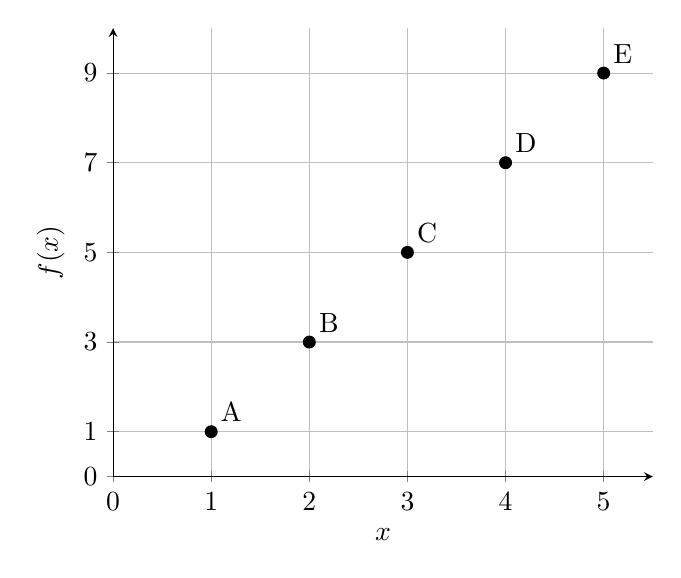
\begin{tikzpicture}
    \begin{axis}[
        grid=major, xlabel = $x$, ylabel = $f(x)$, xmin = 0,
        xmax = 5.5, ymin = 0, ymax = 10, ytick = {0, 1, 3, 5, 7, 9},
        axis lines = left,
    ],
    \draw[black, fill=black] (1,1) circle[radius=0.75mm] node[above right]{A}
            (2,3) circle[radius=0.75mm] node[above right]{B}
            (3,5) circle[radius=0.75mm] node[above right]{C}
            (4,7) circle[radius=0.75mm] node[above right]{D}
            (5,9) circle[radius=0.75mm] node[above right]{E};
    \end{axis}
\end{tikzpicture}
\end{document}
